%%%%%%%%%%%%%%%%%%%%%%%%%%%%%%%%%%%%%%%%%
% Beamer Presentation
% LaTeX Template
% Version 1.0 (10/11/12)
%
% This template has been downloaded from:
% http://www.LaTeXTemplates.com
%
% License:
% CC BY-NC-SA 3.0 (http://creativecommons.org/licenses/by-nc-sa/3.0/)
%
%%%%%%%%%%%%%%%%%%%%%%%%%%%%%%%%%%%%%%%%%

%----------------------------------------------------------------------------------------
%	PACKAGES AND THEMES
%----------------------------------------------------------------------------------------

\documentclass{beamer}

\mode<presentation> {

\usetheme{Madrid}
\usecolortheme{dolphin}
%\setbeamertemplate{footline} % To remove the footer line in all slides uncomment this line
%\setbeamertemplate{footline}[page number] % To replace the footer line in all slides with a simple slide count uncomment this line

%\setbeamertemplate{navigation symbols}{} % To remove the navigation symbols from the bottom of all slides uncomment this line
}
%\usepackage{xcolor}
\usepackage{graphicx} % Allows including images
\usepackage{ragged2e} % Jusitfy
\usepackage{booktabs} % Allows the use of \toprule, \midrule and \bottomrule in tables
\usepackage{lmodern}
\usepackage{amsfonts}
\usepackage{amsmath}
\usepackage{mathtools}
\usepackage{multicol}
\usepackage{listings} % C++ code
\usepackage{xcolor}
\lstset{language=C++,
                basicstyle=\footnotesize\ttfamily,
                keywordstyle=\footnotesize\color{blue}\ttfamily,
}
\addtobeamertemplate{block begin}{}{\justifying} %Justify
%----------------------------------------------------------------------------------------
%	TITLE PAGE
%----------------------------------------------------------------------------------------

\title[Deques Applications]{Deques Applications} % The short title appears at the bottom of every slide, the full title is only on the title page

\author{Ulises Mdz, Ulises Tirado Zatarain} % Your name

\institute[UTM] % Your institution as it will appear on the bottom of every slide, may be shorthand to save space
{
Algorist Weekly Talks \\ % Your institution for the title page
\medskip
\textit{ulisesmdzmtz@gmail.com}\\ % Your email address
\textit{ulises.tirado@cimat.mx} % Your email address
}
\date{\today} % Date, can be changed to a custom date

\begin{document}

\begin{frame}
\titlepage % Print the title page as the first slide
\end{frame}


%--------------------------------------------------------
%-- OVERVIEW SECTION
%--------------------------------------------------------
\begin{frame}
\frametitle{Overview} % Table of contents slide, comment this block out to remove it
\tableofcontents % Throughout your presentation, if you choose to use 
\end{frame}
%--------------------------------------------------------
%	PRESENTATION SLIDES
%--------------------------------------------------------
\section{Finding Maximum}
\subsection{Problem definition}
\begin{frame}
\frametitle{Finding Maximum}

\begin{block}{Description}
Given an array $\mathbf{nums}$, there is a \textit{sliding window} of size $\mathbf{k}$ which is moving from the very left of the array to the very right. You can only see the $\mathbf{k}$ numbers in the window. Each time the sliding window moves right by one position, can you calculate the maximum element each time the window moves?.
\footnote{Source: \url{https://leetcode.com/problems/sliding-window-maximum/}}
\end{block}
\end{frame}
%--------------------------------------------------------
\subsection{Example}
\begin{frame}
\frametitle{Example/Simulation}
\begin{center}
For example,
Given $\mathbf{nums = [1,3,-1,-3,5,3,6,7]}$, and $\mathbf{k = 3}$.\\
\end{center}
\begin{center}
	\large
    \begin{tabular}{c c c c c c c c c c }
    \multicolumn{8}{ c }{ \textbf{Window position} } & & \textbf{Max} \\
    \cline{1-8} \cline{10-10}
	\textbf{[1} & \textbf{3} & \textbf{-1]} & -3 & 5 & 3 & 6 & 7 & & \textbf{3} \\
    1 & \textbf{[3} & \textbf{-1} & \textbf{-3]} & 5 & 3 & 6 & 7 & & \textbf{3} \\
    1 & 3 & \textbf{[-1} & \textbf{-3} & \textbf{5]} & 3 & 6 & 7 & & \textbf{3} \\
    1 & 3 & -1 & \textbf{[-3} & \textbf{5} & \textbf{3]} & 6 & 7 & & \textbf{5} \\
    1 & 3 & -1 & -3 & \textbf{[5} & \textbf{3} & \textbf{6]} & 7 & & \textbf{6} \\
    1 & 3 & -1 & -3 & 5 & \textbf{[3} & \textbf{6} & \textbf{7]} & & \textbf{7} \\
    \end{tabular}
\end{center}
\begin{center}
	Therefore, return the max sliding window as $\mathbf{[3,3,5,5,6,7]}$.
\end{center}
\end{frame}
%--------------------------------------------------------
\begin{frame}
\Huge{\centerline{ Could you solve it in linear time? }}
\end{frame}
%--------------------------------------------------------
\section{Deque Review} 
\subsection{C++ STL Deque} 
\begin{frame}
\frametitle{C++ STL Deque Review}
\begin{block}{std::dueque}
template $<$ class T, class Alloc = allocator$<$T$>$ $>$ class deque;
\end{block}
\begin{block}{\textbf{Double ended queue}}
\textbf{deque} (usually pronounced like "deck") is an irregular acronym of double-ended queue. Double-ended queues are sequence containers with dynamic sizes that can be expanded or contracted on both ends (either its front or its back).
Specific libraries may implement deques in different ways, generally as some form of dynamic array. But in any case, they allow for the individual elements to be accessed directly through random access iterators, with storage handled automatically by expanding and contracting the container as needed.
Therefore, they provide a functionality similar to vectors, but with efficient insertion and deletion of elements also at the beginning of the sequence, and not only at its end. 
\end{block}
\end{frame}
%--------------------------------------------------------
\subsection{Hints}
\begin{frame}
\frametitle{ Some things to notice }
\begin{itemize}
	\item What happens when we insert an element?
	\item What happens when we remove an element?
	\item What kind of data structure do we need?
	\item Do we need to store all elements from window?
	\item What we need to store data or index?
	\item How to know if some element belongs to some window?
	\item Useful elements
\end{itemize}
\end{frame}
%--------------------------------------------------------
\begin{frame}
\frametitle{ Solution }
\begin{block}{Using Deque}
We create a \textbf{Deque}, $\mathbf{Q_i}$ of capacity $\mathbf{k}$, that stores only \textit{useful elements} of current window of $\mathbf{k}$ elements. \textbf{An element is useful} if it is in current window and is greater than all other elements on left side of it in current window. We process all array elements one by one and maintain $\mathbf{Qi}$ to contain useful elements of current window and these useful elements are maintained in sorted order. The element at front of the $\mathbf{Qi}$ is the largest and element at rear of $\mathbf{Qi}$ is the smallest of current window.
\end{block}
\end{frame}
%--------------------------------------------------------
\begin{frame}
\subsection{Algorithm}
\frametitle{ Solution Algorithm }
\begin{block}{Algorithm}
\begin{itemize}
	\item Process first $\mathbf{k}$ (or first window) elements of array.
	\begin{enumerate}
		\item For very element, the previous smaller elements are useless so remove them from $\mathbf{Qi}$ (Remove form rear).
		\item Add new element at rear of queue.
	\end{enumerate}
	\item  Process rest of the elements, i.e., from $\mathbf{k}$ to $\mathbf{n-1}$.
	\begin{enumerate}
		\item The element at the front of the queue is \textbf{the largest element} of previous window, so print it.
		\item Remove the elements which are out of this window.
		\item Remove useless elements (all elements smaller than the currently being added).
		\item Add current element at the rear of $\mathbf{Qi}$.
	\end{enumerate}
	\item Print the maximum element of last window
\end{itemize}
Full source code: \url{http://ideone.com/3a3rs9}
\end{block}
\end{frame}
%--------------------------------------------------------
\subsection{Visualization}
\begin{frame}
\frametitle{Visualization}
\begin{figure}
	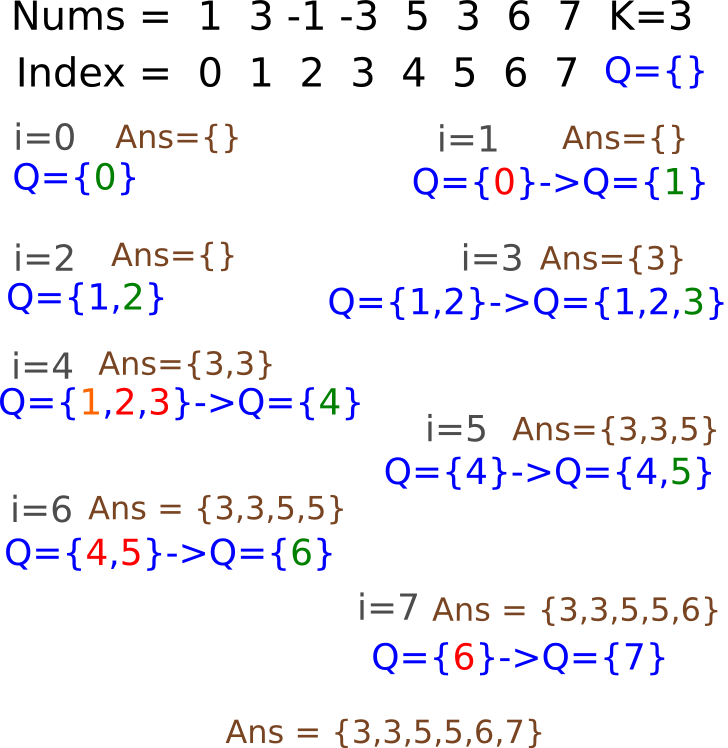
\includegraphics[width=0.55\linewidth]{k_max.png}
	\caption{Algorithm to find maximum value on  a slide window}
\end{figure}
\end{frame}
%--------------------------------------------------------
\subsection{ Code Implementation (C++) }
\begin{frame}[fragile]
\frametitle{ Code Implementation (C++) }
\begin{example}[ C++ Implementation ]
\begin{lstlisting}
void printKMax(int arr[], int n, int k) {
   deque<int>  Qi;
   for(int i=0; i<k; ++i) {
      while ( (!Qi.empty()) && arr[i] >= arr[Qi.back()])
         Qi.pop_back();
      Qi.push_back(i);
   }
   for(int i=k; i<n; ++i) {
      cout << arr[Qi.front()] << " ";
      while((!Qi.empty()) && Qi.front() <= (i-k))
         Qi.pop_front();
      while((!Qi.empty()) && arr[i]>=arr[Qi.back()])
         Qi.pop_back();
      Qi.push_back(i);
    }
    cout << arr[Qi.front()];
}
\end{lstlisting}
\end{example}
\end{frame}
%--------------------------------------------------------
\begin{frame}
\Huge{\centerline{ Q \& A }}
\normalsize
\begin{block}{Other solutions using DP}
\begin{itemize}
	\item \url{http://stackoverflow.com/a/17249084}
	\item \url{http://www.zrzahid.com/sliding-window-minmax/}
\end{itemize}
\end{block}
\end{frame}
%--------------------------------------------------------
%--------------------------------------------------------
%--------------------------------------------------------
%--------------------------------------------------------
%--------------------------------------------------------
%--------------------------------------------------------
%--------------------------------------------------------
%--------------------------------------------------------
%--------------------------------------------------------
%--------------------------------------------------------
%--------------------------------------------------------
\section{ Deque \& BFS}
\subsection{BFS 0/1}
\begin{frame}
\frametitle{BFS 0/1}

\begin{block}{Ocean Currents (Difficult)}
At each location, the current  owes in some direction. The captain can choose to either go with the
 ow of the current, using no energy, or to move one square in any other direction, at the cost of one
energy unit. The boat always moves in one of the following eight directions: north, south, east, west,
north-east, Northwest, south-east, south-west. The boat cannot leave the boundary of the lake.\\

\textbf{You are to help him devise a strategy to reach the destination with the minimum energy consumption.}
\end{block}

\end{frame}
%--------------------------------------------------------
\begin{frame}
\frametitle{ References }
\begin{itemize}
	\item \url{http://www.cplusplus.com/reference/queue/}
	\item \url{https://en.wikipedia.org/}
	\item \url{http://www.geeksforgeeks.org/maximum-of-all-subarrays-of-size-k/}
	\item \url{https://chococontest.wordpress.com/category/bfs-01/}
	\item \url{http://ideone.com/PvCked}
\end{itemize}
\end{frame}

\end{document} 
